\documentclass[tikz,border=8pt]{standalone}
% Shared look for every TikZ diagram. Load with % Shared look for every TikZ diagram. Load with % Shared look for every TikZ diagram. Load with \input{../../tools/tikz-style.tex}
\usepackage[T1]{fontenc}
\usepackage{lmodern}
\renewcommand{\sfdefault}{lmr}  % diagrams use the same serif as the text
\usetikzlibrary{arrows.meta, positioning, shapes.geometric, calc, fit, backgrounds}
\definecolor{cblue}{HTML}{4C78A8}
\definecolor{corange}{HTML}{F58518}
\definecolor{cgreen}{HTML}{54A24B}
\definecolor{cred}{HTML}{E45756}
\definecolor{cpurple}{HTML}{B279A2}
\definecolor{cgrey}{HTML}{6B6B6B}
\tikzset{
  every picture/.style={font=\sffamily, line width=1.2pt},
  box/.style={draw=#1, fill=#1!12, rounded corners=4pt, align=center, inner sep=7pt, minimum height=1.1cm},
  box/.default=cgrey,
  arrow/.style={-{Stealth[length=3mm]}, draw=cgrey, line width=1.4pt},
  title/.style={font=\sffamily\bfseries\Large},
  note/.style={font=\sffamily\small, text=cgrey, align=center},
}
\AtBeginDocument{\hyphenpenalty=10000 \exhyphenpenalty=10000}

\usepackage[T1]{fontenc}
\usepackage{lmodern}
\renewcommand{\sfdefault}{lmr}  % diagrams use the same serif as the text
\usetikzlibrary{arrows.meta, positioning, shapes.geometric, calc, fit, backgrounds}
\definecolor{cblue}{HTML}{4C78A8}
\definecolor{corange}{HTML}{F58518}
\definecolor{cgreen}{HTML}{54A24B}
\definecolor{cred}{HTML}{E45756}
\definecolor{cpurple}{HTML}{B279A2}
\definecolor{cgrey}{HTML}{6B6B6B}
\tikzset{
  every picture/.style={font=\sffamily, line width=1.2pt},
  box/.style={draw=#1, fill=#1!12, rounded corners=4pt, align=center, inner sep=7pt, minimum height=1.1cm},
  box/.default=cgrey,
  arrow/.style={-{Stealth[length=3mm]}, draw=cgrey, line width=1.4pt},
  title/.style={font=\sffamily\bfseries\Large},
  note/.style={font=\sffamily\small, text=cgrey, align=center},
}
\AtBeginDocument{\hyphenpenalty=10000 \exhyphenpenalty=10000}

\usepackage[T1]{fontenc}
\usepackage{lmodern}
\renewcommand{\sfdefault}{lmr}  % diagrams use the same serif as the text
\usetikzlibrary{arrows.meta, positioning, shapes.geometric, calc, fit, backgrounds}
\definecolor{cblue}{HTML}{4C78A8}
\definecolor{corange}{HTML}{F58518}
\definecolor{cgreen}{HTML}{54A24B}
\definecolor{cred}{HTML}{E45756}
\definecolor{cpurple}{HTML}{B279A2}
\definecolor{cgrey}{HTML}{6B6B6B}
\tikzset{
  every picture/.style={font=\sffamily, line width=1.2pt},
  box/.style={draw=#1, fill=#1!12, rounded corners=4pt, align=center, inner sep=7pt, minimum height=1.1cm},
  box/.default=cgrey,
  arrow/.style={-{Stealth[length=3mm]}, draw=cgrey, line width=1.4pt},
  title/.style={font=\sffamily\bfseries\Large},
  note/.style={font=\sffamily\small, text=cgrey, align=center},
}
\AtBeginDocument{\hyphenpenalty=10000 \exhyphenpenalty=10000}

\begin{document}
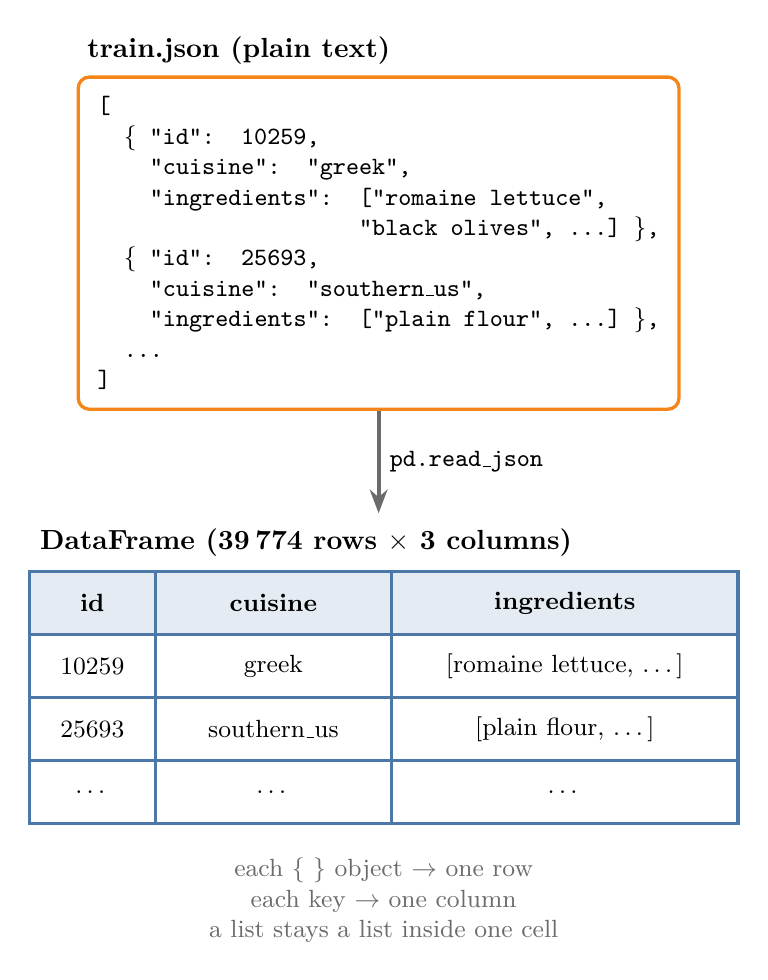
\begin{tikzpicture}
  \node[box=corange, fill=white, align=left, font=\ttfamily\small, anchor=north west] (j) at (0,0) {%
[\\
\ \ \{\ "id": 10259,\\
\ \ \ \ "cuisine": "greek",\\
\ \ \ \ "ingredients": ["romaine lettuce",\\
\ \ \ \ \ \ \ \ \ \ \ \ \ \ \ \ \ \ \ \ "black olives", ...]\ \},\\
\ \ \{\ "id": 25693,\\
\ \ \ \ "cuisine": "southern\_us",\\
\ \ \ \ "ingredients": ["plain flour", ...]\ \},\\
\ \ ...\\
]};
  \node[anchor=south west, font=\sffamily\bfseries] at (j.north west) {train.json (plain text)};
  \begin{scope}[shift={(-0.6,-6.7)}, cell/.style={draw=cblue, minimum height=0.8cm, font=\small, inner sep=2pt}]
    \foreach \x/\w/\t in {0.8/1.6/id, 3.1/3.0/cuisine, 6.8/4.4/ingredients}
      \node[cell, fill=cblue!15, font=\small\bfseries, minimum width=\w cm] at (\x,0) {\t};
    \foreach \y/\a/\b/\c in {-0.8/10259/greek/{[romaine lettuce, \dots]},
                             -1.6/25693/southern\_us/{[plain flour, \dots]}, -2.4/{\dots}/{\dots}/{\dots}} {
      \node[cell, minimum width=1.6cm] at (0.8,\y) {\a};
      \node[cell, minimum width=3.0cm] at (3.1,\y) {\b};
      \node[cell, minimum width=4.4cm] at (6.8,\y) {\c};
    }
    \node[anchor=south west, font=\sffamily\bfseries] at (0,0.45) {DataFrame (39\,774 rows $\times$ 3 columns)};
    \node[note, anchor=north] at (4.5,-3.1) {each \{ \} object $\rightarrow$ one row\\each key $\rightarrow$ one column\\a list stays a list inside one cell};
  \end{scope}
  \draw[arrow] (j.south) -- node[right, font=\ttfamily\small]{pd.read\_json} ++(0,-1.3);
\end{tikzpicture}
\end{document}
